% Written by Daina Chiba (daina.chiba@gmail.com).
% It was mostly copied from two poster style files:
% beamerthemeI6pd2.sty written by
%	 	Philippe Dreuw <dreuw@cs.rwth-aachen.de> and
% 		Thomas Deselaers <deselaers@cs.rwth-aachen.de>
% and beamerthemeconfposter.sty written by
%     Nathaniel Johnston (nathaniel@nathanieljohnston.com)
%		http://www.nathanieljohnston.com/2009/08/latex-poster-template/
% ---------------------------------------------------------------------------------------------------%
% Preamble
% ---------------------------------------------------------------------------------------------------%
\documentclass[final]{beamer}
\usepackage[orientation=landscape,size=custom,width=110,height=86,scale=1.2,debug]{beamerposter}
\mode<presentation>{\usetheme{RicePoster}}
\usepackage[english]{babel}
\usepackage[latin1]{inputenc}
\usepackage[T1]{fontenc}
\usepackage{amsmath,amsthm, amssymb, latexsym}
\usepackage[demo]{graphicx}
\usepackage{subfig}

\usepackage{array,booktabs,tabularx}
\newcolumntype{Z}{>{\centering\arraybackslash}X} % centered tabularx columns


%   Begin Additional Packages
\usepackage{blindtext}
\usepackage{graphicx}
\usepackage{tikz}
%   End Additional Packages


% comment
\newcommand{\comment}[1]{}

\newlength{\columnheight}
\setlength{\columnheight}{80cm}
\newlength{\sepwid}
\newlength{\onecolwid}
\newlength{\twocolwid}
\newlength{\threecolwid}
\newlength{\restofpage}
\setlength{\sepwid}{0.024\paperwidth}
\setlength{\onecolwid}{0.24\paperwidth}
\setlength{\twocolwid}{0.4\paperwidth}
\setlength{\threecolwid}{0.19\paperwidth}
\setlength{\restofpage}{0.7\paperwidth}

% ---------------------------------------------------------------------------------------------------%
% Title, author, date, etc.
% ---------------------------------------------------------------------------------------------------%
\title{\huge Auto Segmentation}
\author{Will LeVine \& Cole Morgan}
\institute[Rice University]{Department of Computer Science, Rice University}
\date[Nov.2018]{November, 2018}
\def\conference{COMP340 Term Project: Automobile Segmentation and Clustering}
\def\yourEmail{wvl1@rice.edu,cmm16@rice.edu}


% ---------------------------------------------------------------------------------------------------%
% Contents
% ---------------------------------------------------------------------------------------------------%
\begin{document}
\begin{frame}[t]

\begin{columns}[t]

\begin{column}{\onecolwid}

  \begin{block}{Background}
    \begin{itemize}
      \item used U.S. car market generates over \$100 billion annually and is quickly growing
      \item used car matching process is inefficient because selective online searches require car attributes to be manually labeled (e.g. color)

    \end{itemize}


  \end{block}

    \vskip5ex

    \begin{block}{Goal}
      \begin{itemize}
        \item reduce inefficiency present in the process of searching in the online used car market, improve user experience
        \item develop method to isolate an image of a car from its surrounding background
        \item train model to cluster groups of cars based off certain features (e.g. color) to expedite the used car searching process

      \end{itemize}
    \end{block}

    \vskip5ex

    \begin{block}{Issues and Where We'd Like To Go}
      \begin{itemize}
        \item would purchase extra compute power so that we could maintain image quality of the cars
          \begin{itemize}
            \item couldn't do that for this project because of limited computing power and financial resources
            \item instead downsampled from the images (more information below)
          \end{itemize}
        \item would extend the clustering algorithm to instead be a recommendation system
        \begin{itemize}
          \item couldn't do that for this project due to the inavailability of user-preference data
        \end{itemize}
      \end{itemize}
    \end{block}

    \vskip5ex

    \begin{block}{Data Downsampling}
        \begin{itemize}
            \item we were limited by memory and computing power
            \item to remedy these issues, we downsampled all the input images and labels from 1918x1280 to 128x128 using Pillow's default image resizing
        \end{itemize}

        \begin{tikzpicture}
          \node[inner sep=0pt] (raw) at (0,-13.5)
              {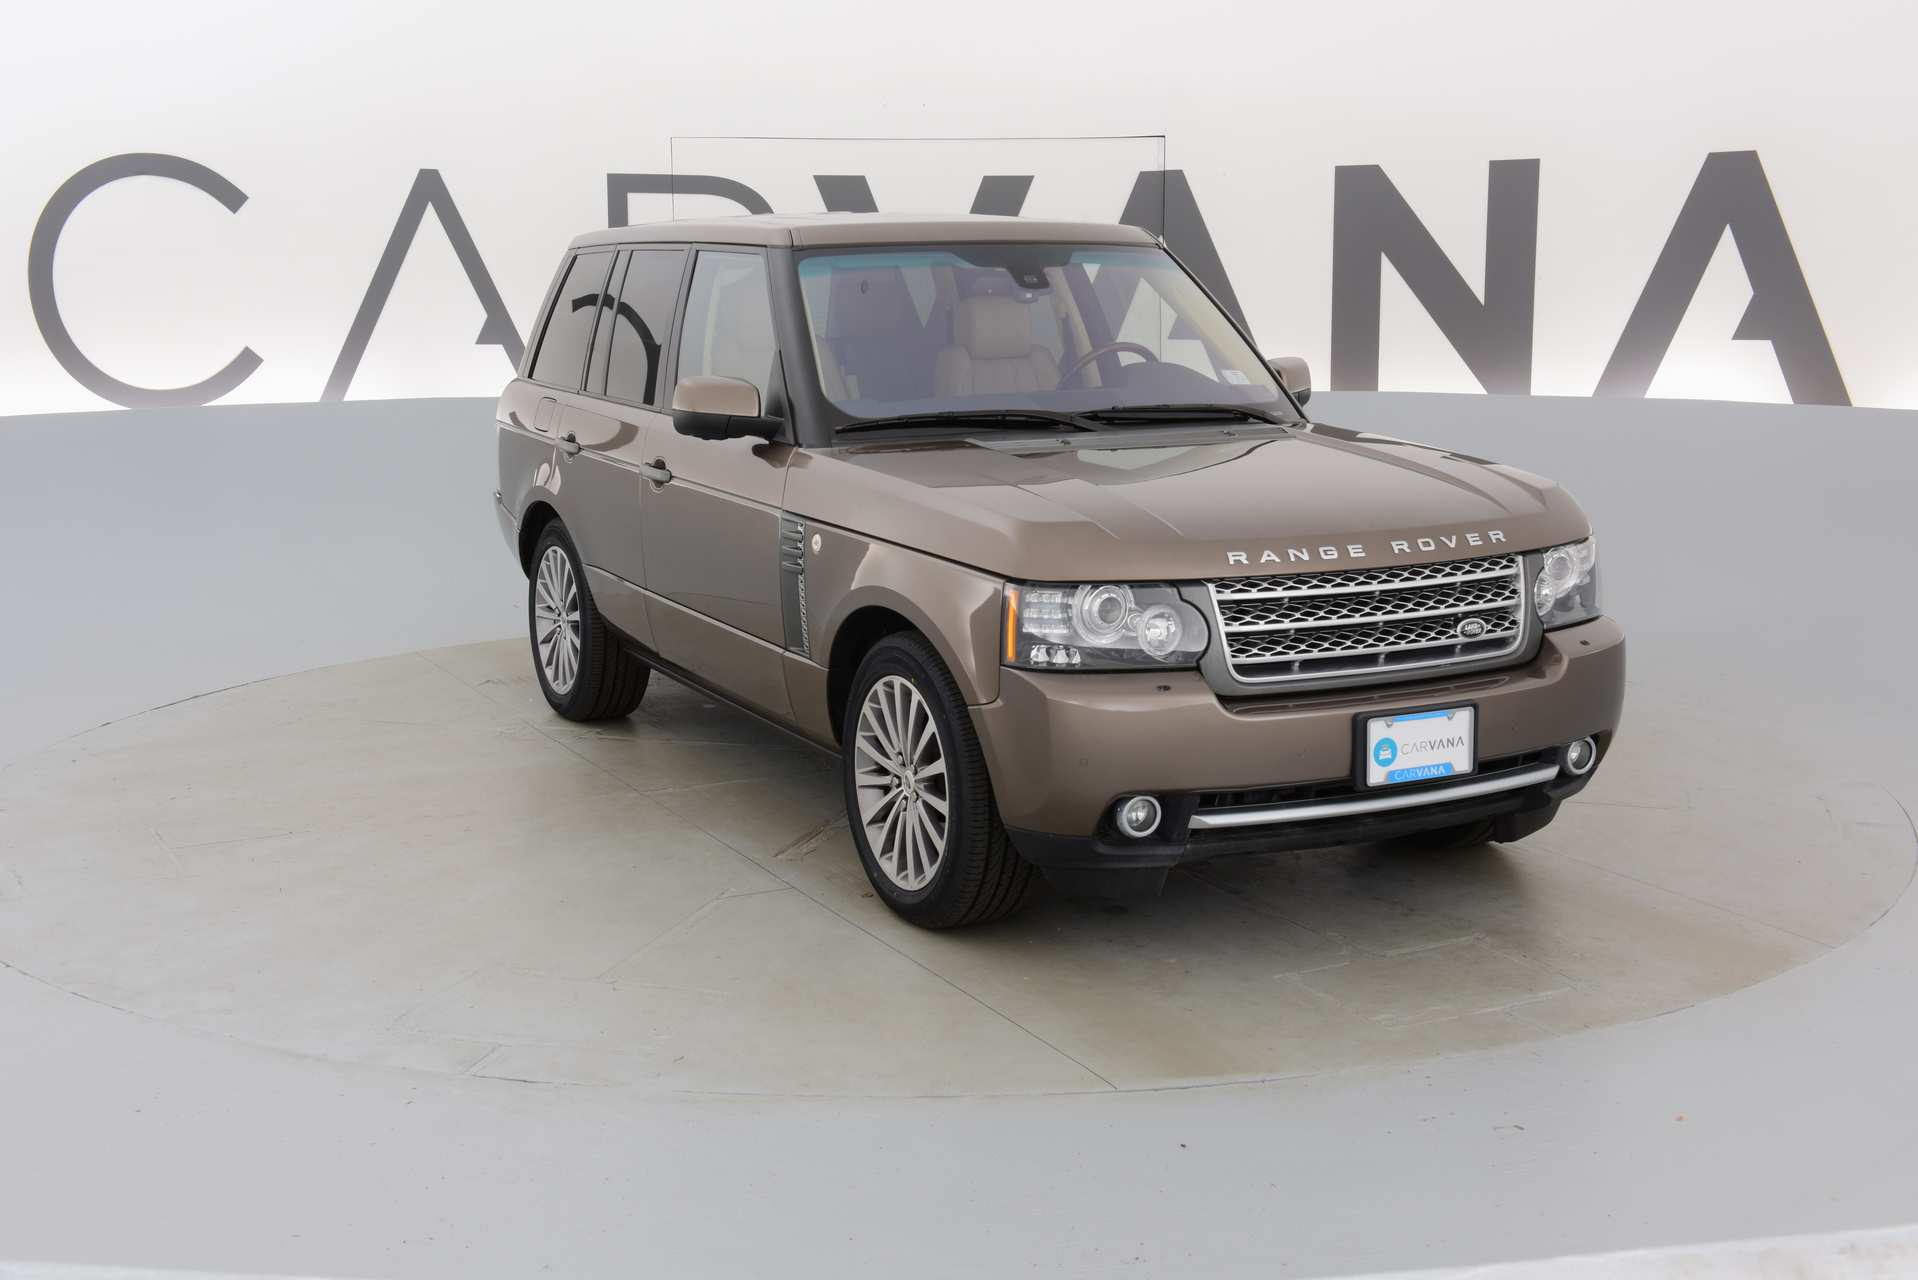
\includegraphics[width=8cm]{./new_figs/raw.jpg}};
          \node[inner sep=0pt] (raw lbl) at (0,-17.5)
              {Original Image};
          \node[inner sep=0pt] (downsample) at (18,-13.5)
              {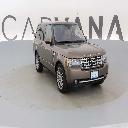
\includegraphics[width=8cm]{./new_figs/downsampled.jpg}};
          \node[inner sep=0pt] (downsample lbl) at (18,-18.5)
              {Downsampled Image};
          \draw[->,line width=4pt] (raw.east) -- (downsample.west);
        \end{tikzpicture}
    \end{block}

\end{column}

% -----------------------------------------------------------
% Start the second column
% -----------------------------------------------------------
\begin{column}{\restofpage}
    \begin{columns}[c]
        \column{0.5\textwidth}
        \begin{block}{UNet}
              \begin{figure}
                  \centering
                  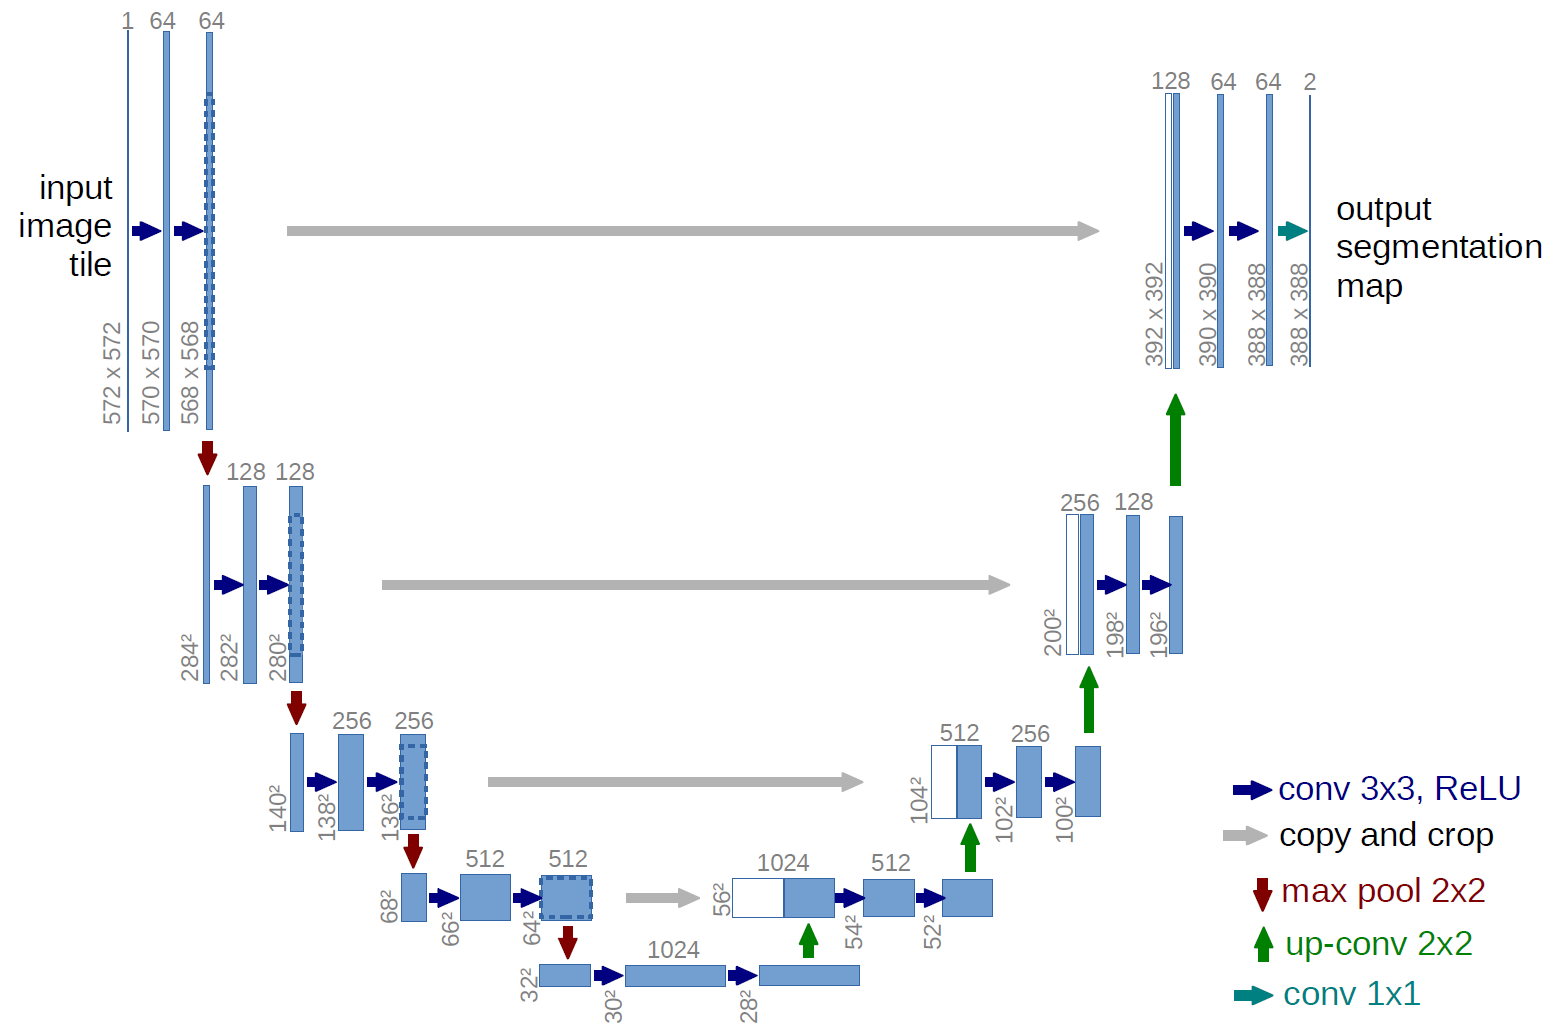
\includegraphics[width=.6\textwidth]{./figs/unet_architecture.png}
                  \caption{UNet Architecture}
              \end{figure}
              \begin{figure}
              \begin{tabular}{cccc}
              \subfloat[UNet Train/Validation Accuracy History]{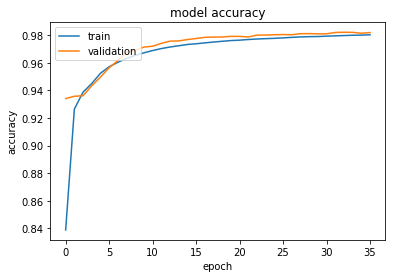
\includegraphics[width = 7in]{./new_figs/train_accuracy_history.png}} &
              \subfloat[UNet Train/Validation Loss History]{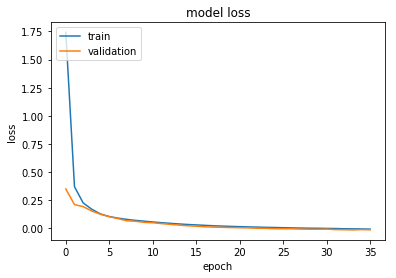
\includegraphics[width = 7in]{./new_figs/train_loss_history.png}}
              \end{tabular}
              \end{figure}
        \end{block}

        \begin{figure}
        \begin{tabular}{cccc}
        \subfloat[Example 1]{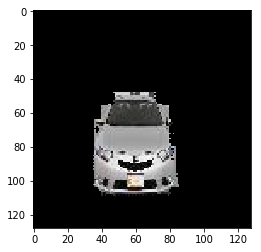
\includegraphics[width = 2.5in]{./new_figs/unet_output1.png}} &
        \subfloat[Example 2]{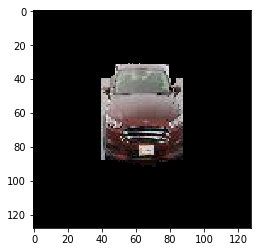
\includegraphics[width = 2.5in]{./new_figs/unet_output2.png}} &
        \subfloat[Example 3]{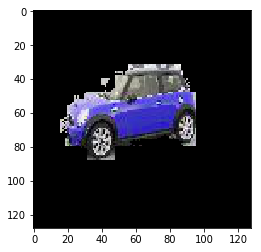
\includegraphics[width = 2.5in]{./new_figs/unet_output3.png}} &
        \subfloat[Example 4]{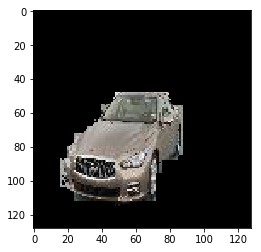
\includegraphics[width = 2.5in]{./new_figs/unet_output4.png}}
        \end{tabular}
        \caption{UNet Output Examples}
        \end{figure}

        \vskip5ex

        \begin{block}{UNet Modifications}
              \begin{itemize}
                \item added Early Stopping callback with patience of 3
                \item added 9 dropout layers with hyperparameter of .5 (per suggestion of Geoff Hinton) to reduce overfitting
                  \begin{itemize}
                    \item Train F1: 0.966
                    \item Test F1: 0.966
                  \end{itemize}
                \item added batch normalization to all 2D convolution blocks to unify feature scales
                \begin{itemize}
                  \item training F1
                  \begin{itemize}
                    \item without batch normalization: 0.876
                    \item with batch noramlization: 0.966
                  \end{itemize}
                  \item testing F1
                  \begin{itemize}
                    \item without batch normalization: 0.831
                    \item with batch noramlization: 0.966
                  \end{itemize}
                \end{itemize}
              \end{itemize}
        \end{block}

        \column{0.5\textwidth}
        \begin{block}{Example Clustering Method: \newline Automobile Color}

            \centering
            \begin{itemize}
              \item Goal: cluster automobiles based on RGB values. Used car sites provide search narrowing through color selection, so we would like to provide a serivce that autonomously identifies the color of the car
              \item Issue: RGB values are distributed in lines radiating from the origin
              \item Solution: Cluster based off of RGB ratios
              \begin{tikzpicture}
                \node[inner sep=0pt] (raw) at (0,-13.5)
                    {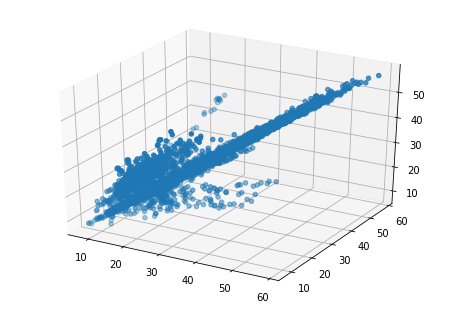
\includegraphics[width=15cm]{./new_figs/colors_3d.png}};
                \node[inner sep=0pt] (raw lbl) at (0,-19.5)
                    {RGB Plot};
                \node[inner sep=0pt] (features) at (18,-13.5)
                    {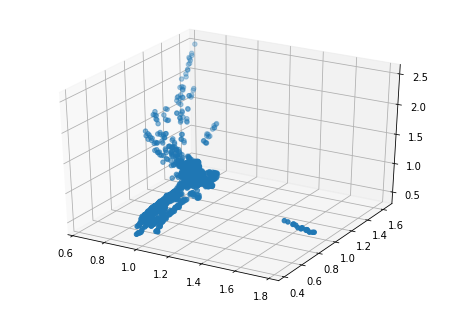
\includegraphics[width=15cm]{./new_figs/color_ratios_3d.png}};
                \node[inner sep=0pt] (features lbl) at (18,-19.5)
                    {RGB Ratio Plot};
                \draw[->,line width=4pt] (raw.east) -- (features.west);
              \end{tikzpicture}

            \end{itemize}
        \end{block}

        \begin{block}{Clustering Approach}
          \begin{itemize}
            \item we used DBSCAN on the RGB ratios
              \begin{itemize}
                \item we wanted the algorithm to be able to select the number of colors because we were unsure of how many colors there were in the dataset
                \item we wanted to the algorithm to be able to identify when a data point is noise to alert the user that they must label the color of the car because the algorithm is unsure
              \end{itemize}
            \item Number of Clusters: 12
            \item Number of Noise Points: 699 out of 5088
          \end{itemize}
        \end{block}

        \begin{block}{Clustering Examples}
          \begin{figure}
          \begin{tabular}{cccc}
          \subfloat[Blue 1]{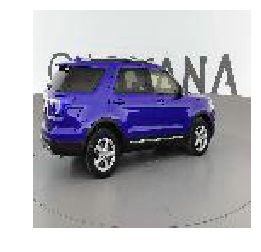
\includegraphics[width = 2.5in]{./new_figs/blue_1.png}} &
          \subfloat[Blue 2]{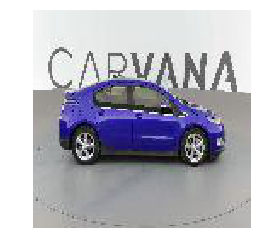
\includegraphics[width = 2.5in]{./new_figs/blue_2.png}} &
          \subfloat[Blue 3]{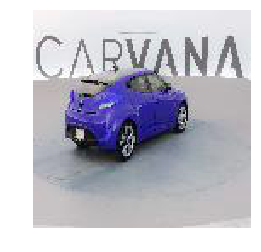
\includegraphics[width = 2.5in]{./new_figs/blue_3.png}} &
          \subfloat[Blue 4]{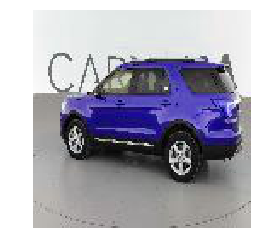
\includegraphics[width = 2.5in]{./new_figs/blue_4.png}}\\
          \subfloat[Orange 1]{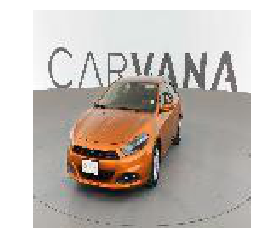
\includegraphics[width = 2.5in]{./new_figs/orange_1.png}} &
          \subfloat[Orange 2]{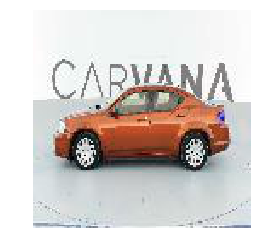
\includegraphics[width = 2.5in]{./new_figs/orange_2.png}} &
          \subfloat[Orange 3]{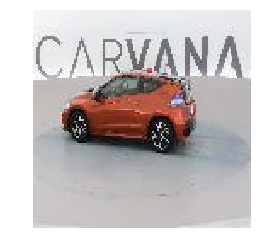
\includegraphics[width = 2.5in]{./new_figs/orange_3.png}} &
          \subfloat[Orange 4]{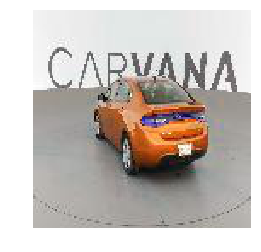
\includegraphics[width = 2.5in]{./new_figs/orange_4.png}}\\
          \subfloat[Beige 1]{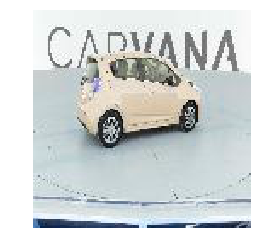
\includegraphics[width = 2.5in]{./new_figs/beige_2.png}} &
          \subfloat[Beige 2]{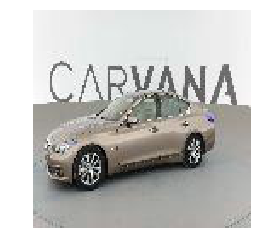
\includegraphics[width = 2.5in]{./new_figs/beige_1.png}} &
          \subfloat[Beige 3]{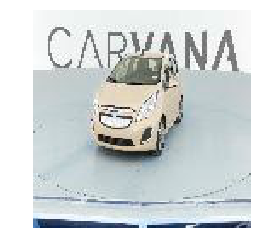
\includegraphics[width = 2.5in]{./new_figs/beige_3.png}} &
          \subfloat[Beige 4]{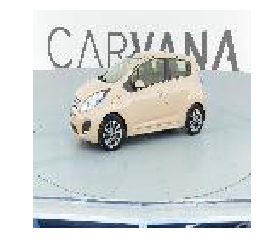
\includegraphics[width = 2.5in]{./new_figs/beige_4.png}}\\
          \subfloat[Brown 1]{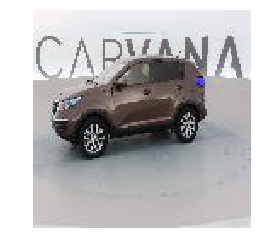
\includegraphics[width = 2.5in]{./new_figs/brown_1.png}} &
          \subfloat[Brown 2]{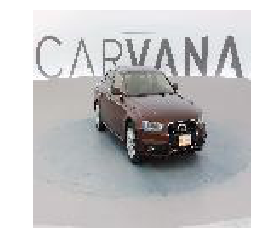
\includegraphics[width = 2.5in]{./new_figs/brown_2.png}} &
          \subfloat[Brown 3]{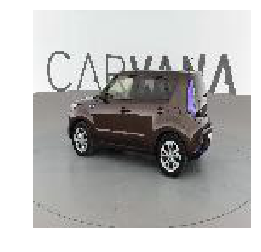
\includegraphics[width = 2.5in]{./new_figs/brown_3.png}} &
          \subfloat[Brown 4]{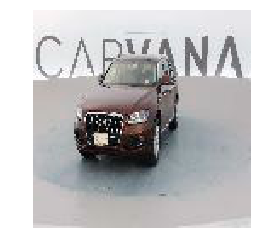
\includegraphics[width = 2.5in]{./new_figs/brown_4.png}}
          \end{tabular}
          \caption{Example Color Clusters. Each row corresponds to a cluster}
          \end{figure}
        \end{block}


    \end{columns}

\end{column}

\end{columns}

\end{frame}
\end{document}
